\chapter{Result}\label{Ch:Result}

Figure~\ref{FIG:before_refinement} shows some examples of result before the data refinement steps were applied. The results seems to contain some face-like objects, but the original faces in the sketch images were not properly translated, resulting in weired colorization in the result. The result of photograph to sketch translation also shows severe artifacts due to the mismatch of locations of faces between datasets.

\begin{figure}[ht]
    \begin{center}
    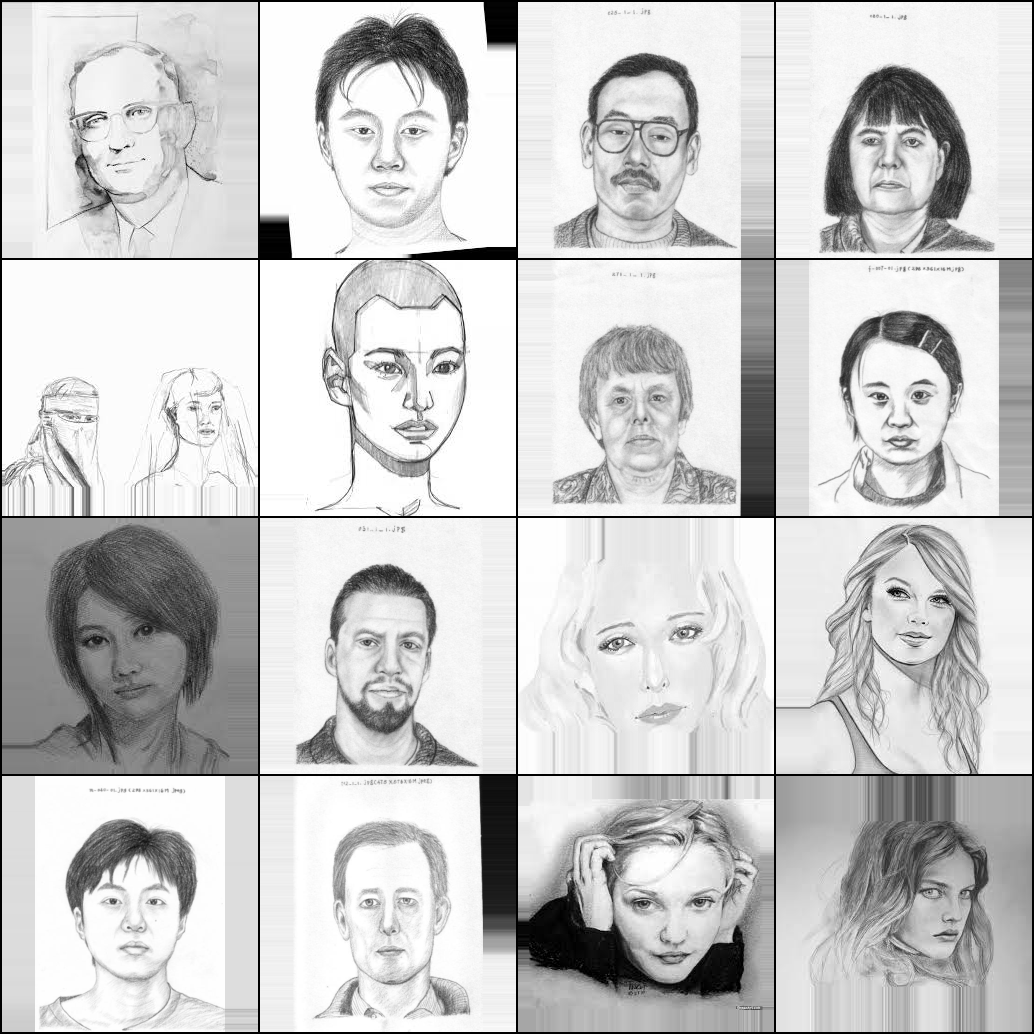
\includegraphics[scale=0.16]{Graphics/ske2pic_origin_before_clean.png}
    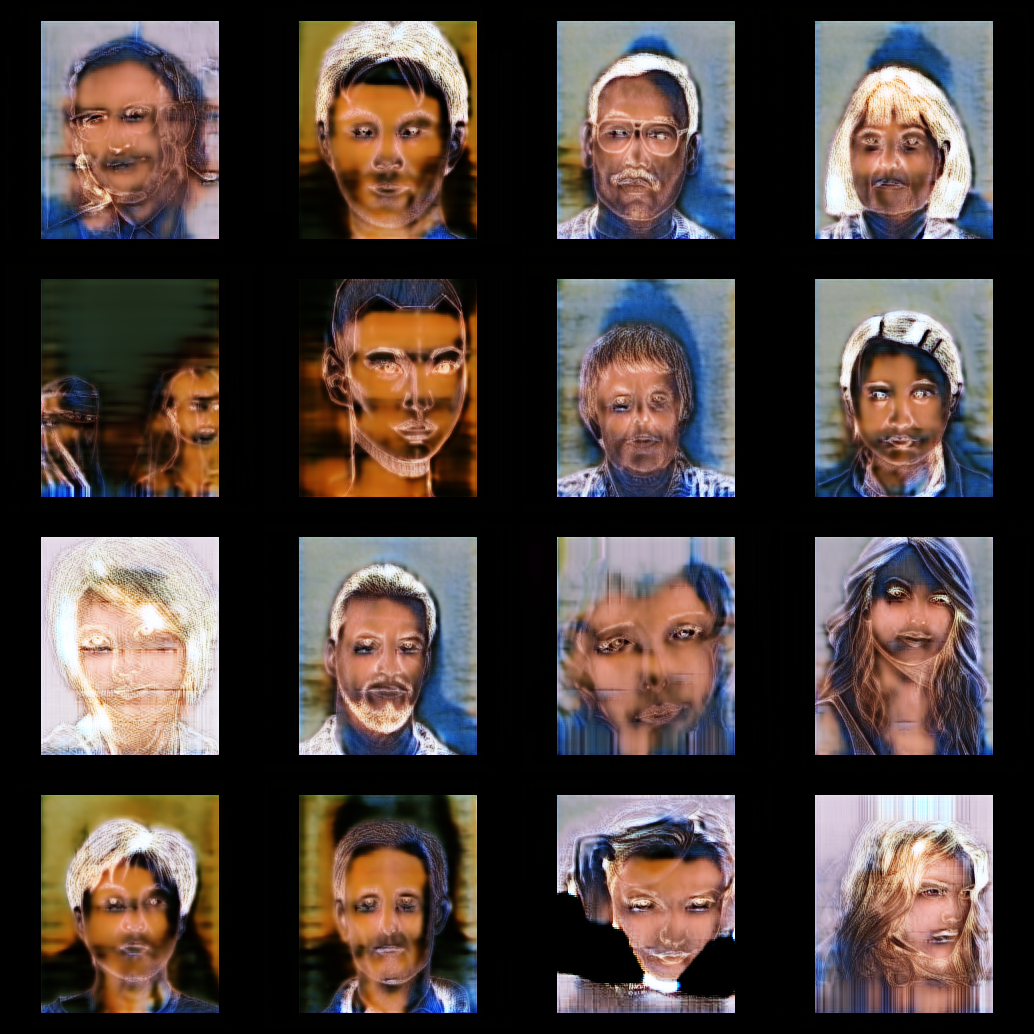
\includegraphics[scale=0.16]{Graphics/ske2pic_result_before_clean.png}

    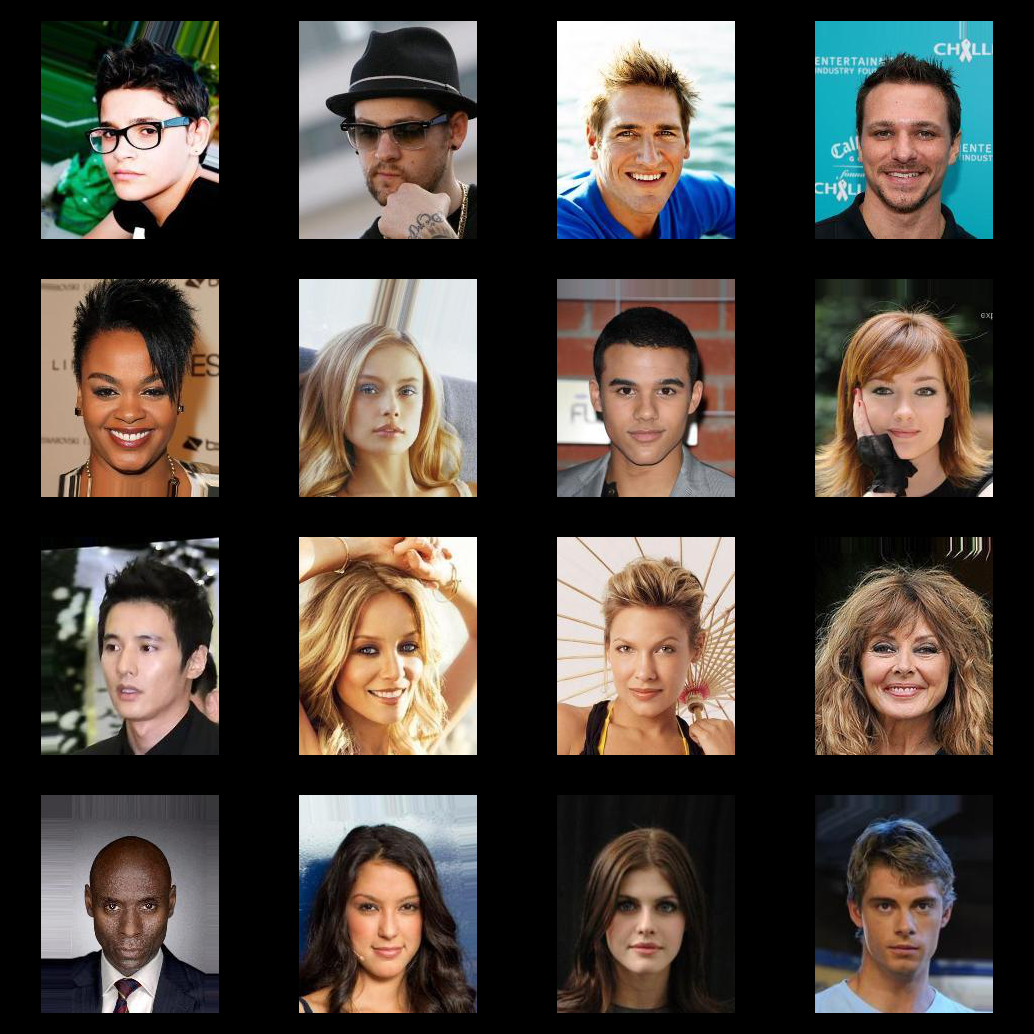
\includegraphics[scale=0.16]{Graphics/pic2ske_origin_before_clean.png}
    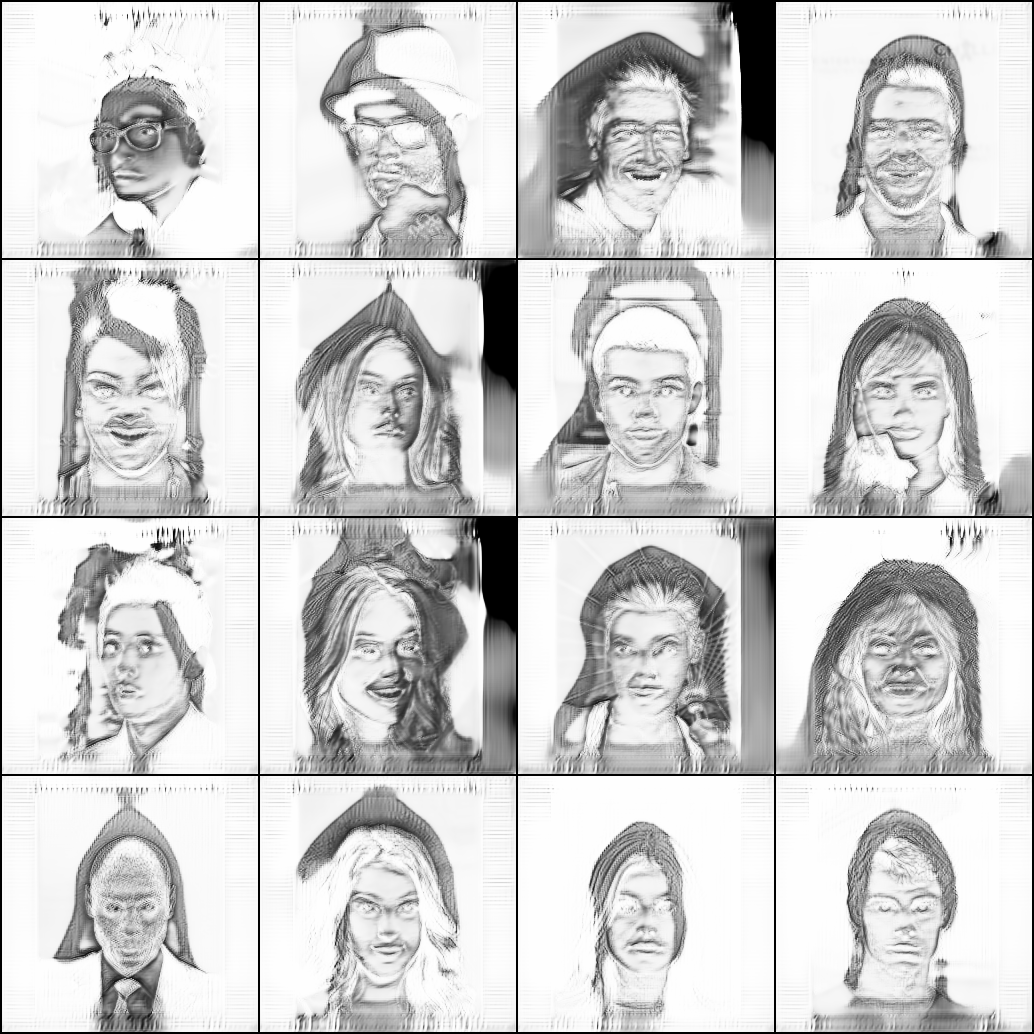
\includegraphics[scale=0.16]{Graphics/pic2ske_result_before_clean.png}
    \end{center}
    \caption{Original input images(left) and result of translations(right) by networks trained before input data is not aligned. Image size is 256 by 256 and model is trained for 64 epochs.}\label{FIG:before_refinement}
\end{figure}

The result seems to be improved considerably with preprocessing steps. Fig~\ref{FIG:smile} shows aligned faces helped the model tell the face and background apart, resulting it to generate better volumes, colors on the paintings. 

\begin{figure}[ht]
    \begin{center}
    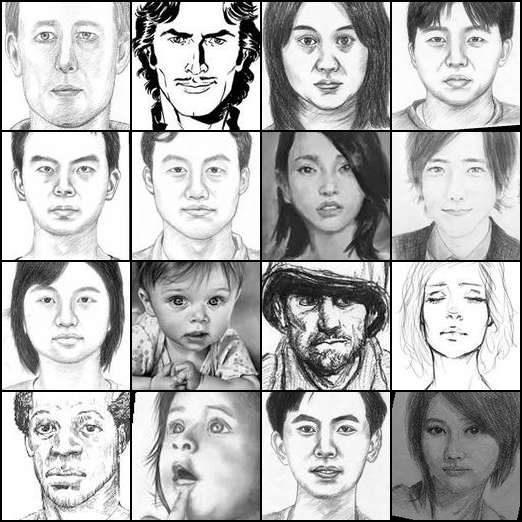
\includegraphics[scale=0.32]{Graphics/smiling_input.png}
    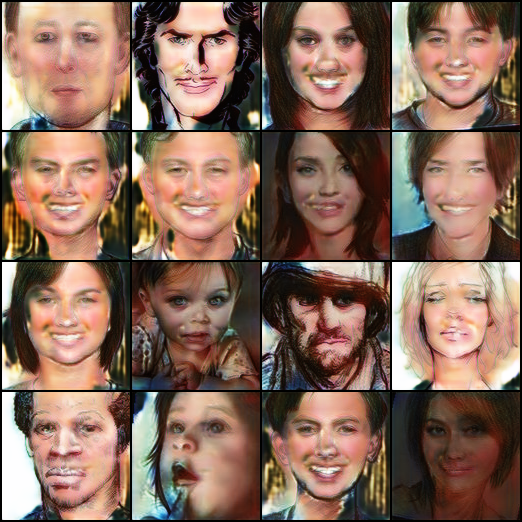
\includegraphics[scale=0.32]{Graphics/smiling_output.png}
    \end{center}
    \caption{Original input images(left) and result of translations(right) by networks trained on datasets after face alignment, but before number of smiling faces was reduced. Image size is 128 by 128 and model is trained for 128 epochs.}\label{FIG:smile}
\end{figure}

However, the results still looks not realistic, mostly due to mistakenly generated smile on the translated images. After some investigation we could find out that is due to the difference of distribution of train data that people smiled much more on the photos rather than on the paintings.
After reducing the ratio of smile in the photograph dataset used as in previous chapter~\ref{Ch:process_data}, we could get following results~\ref{FIG:final}.

\begin{figure}[ht]
    \begin{center}
    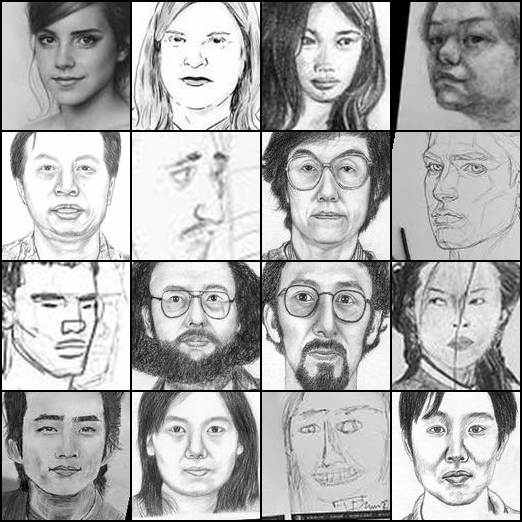
\includegraphics[scale=0.32]{Graphics/ske2pic_origin_final.png}
    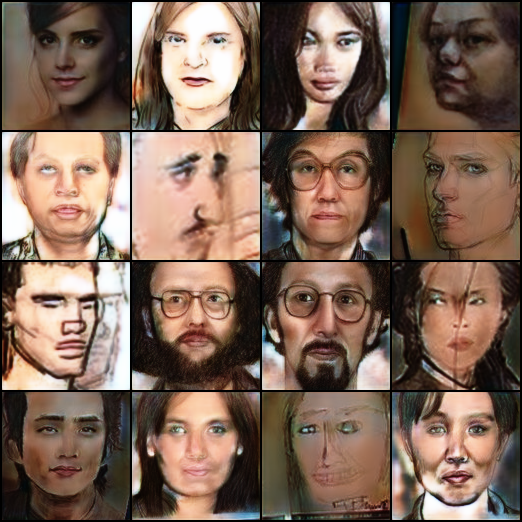
\includegraphics[scale=0.32]{Graphics/ske2pic_result_final.png}

    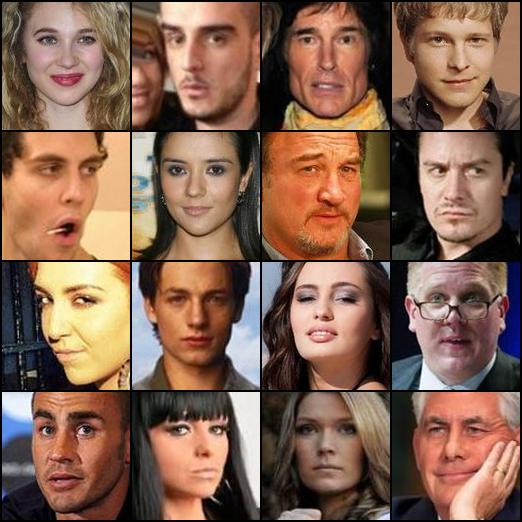
\includegraphics[scale=0.32]{Graphics/pic2ske_origin_final.png}
    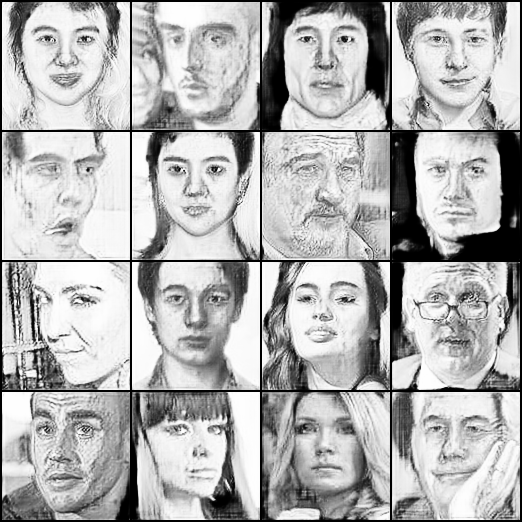
\includegraphics[scale=0.32]{Graphics/pic2ske_result_final.png}
    \end{center}
    \caption{Original input images(left) and result of translations(right) by networks trained on datasets after face alignment and number of smiling faces was reduced. Image size is 128 by 128 and model is trained for 128 epochs.}\label{FIG:final}
\end{figure}

While some of the sketch-to-photo results seems quite realistic(\nth{3} image of \nth{2} column, \nth{2}, \nth{3} of \nth{3}), images generated from low-quality inputs does not seems to be properly translated(\nth{2} image of \nth{2} column, last ones in \nth{3}, \nth{4} column). 
On the other hand, despite the general quality looks fine, some of results(\nth{1}, \nth{2} diagonal positions) resembles average sample images of CUFS datasets rather than contents of input.

% TODO: move to conclusion?
Considering the quantity and quality of sketch images collected from google image search, this amount of dependency on input might be considered acceptible.

We have also tried to replace batch normalization by instance normalization to improve the training quality, but the results are not so satisfactory as shown in \ref{%TODO: add photo}
THe mode collapse problem indicates that instance normalization causes instability of training in this case.




\endinput
